\documentclass{article}

\usepackage[brazil]{babel}

\usepackage[letterpaper,top=2cm,bottom=2cm,left=3cm,right=3cm,marginparwidth=1.75cm]{geometry}
\usepackage{amsmath}
\usepackage{graphicx}
\usepackage[colorlinks=true, allcolors=blue]{hyperref}
\usepackage{caption}
\usepackage{float}
\usepackage{csquotes}

\sloppy

\begin{document}

\begin{titlepage}
    \begin{center}
        {\large Universidade Federal de Minas Gerais}\\[0.2cm]
        {\large Instituto de Ciências Exatas}\\[0.2cm]
        {\large Departamento de Ciência da Computação}\\[0.2cm]
        {\large Projeto Final da disciplina de Aprendizado Descritivo}\\[5.1cm]
        {\large \bf Mineração de dados de eventos em futebol}\\[5.1cm]
    \end{center}
    {\large Alunos: Luís Felipe Ramos Ferreira, Igor Lacerda Faria da Silva,
    Matheus Tiago Pimenta de Souza}\\[0.7cm]
    {\large Professor: Renato Vimieiro}\\[5.1cm]
    \begin{center}
        {\large Belo Horizonte - Minas Gerais}\\[0.2cm]
        {\large 2024}
    \end{center}
\end{titlepage}

\newpage
\begin{quote}
    wabba labba dub dub
\end{quote}

\newpage
\renewcommand{\contentsname}{Sumário}
\tableofcontents
\newpage

\title{Mineração de dados de evento em futebol}
\author{Luís Felipe Ramos Ferreira \\  Igor Lacerda iFaria da Silva \\ Matheus
    Tiago Pimenta de Souza}

\maketitle

\section{Introdução}

O uso de ciência de dados e estatística para analisar esportes é algo que vem
crescendo cada vez mais nos últimos anos. Em
particular, o futebol têm sido um desses
esportes~\cite{takvorian2021beautiful}. A própria UFMG ofertou no
ano passado e novamente neste semestre a disciplina `Ciência de Dados aplicada
ao futebol', o que mostra a relevância do tema. Diversas empresas que atuam na
área surgem a cada dia, e os times de futebol, no Brasil e no resto do
mundo, estão investimento em seus departamentos de dados e estatística.

Nesse sentido, nosso grupo optou por estudar e compreender melhor como funciona
o uso de análises estatísticas no futebol, dado o interesse geral pelo esporte,
e, para isso, nos propusemos a aplicar algoritmos de mineração de dados em
dados futebolísticos, sendo eles dados de súmula, dados de eventos ou até mesmo
dados de
\textit{tracking} dos jogadores, para compreender como as informações acerca do
jogo estão contidas dentro dos dados coletados e como isso pode ser utilizado a
favor das equipes.

Os dados de eventos, especialmente, costumam ser mais fáceis de lidar e mais
fáceis de acessar do que dados de \textit{tracking}, enquanto trazem muito mais
informações do que dados de súmula. Existem, atualmente, algumas bases
gratuitas de dados de evento de partidas, disponibilizadas por diferentes
empresas como \textit{Wyscout} e \textit{StasBomb}. Como a ideia é ter um
panorama geral de diversas partidas, campeonatos e jogadores, iremos utilizar
as bases de dados disponibilizadas sobre as 5 grandes ligas de futebol europeu
das temporadas 17/18 da empresa \textit{Wyscout}.

\subsection{Base de dados}

As bases de dados utilizadas na ferramenta consistirá na base principal
disponibilizada pela empresa \textit{Wyscout},
consistindo em uma base de dados de evento das 5 grandes ligas europeias na
temporada 17/18.

Cada empresa fornecedora de dados possuem seu próprio formato de representação
dos dados de evento. De modo a facilitar a mesclagem entre as bases de dados
utilizadas, iremos converter os dados coletados para uma representação geral
proposta por pesquisadores denominada
\href{https://socceraction.readthedocs.io/en/latest/documentation/spadl/spadl.html}{SPADL}.
A SPADL é uma boa escolha por ser uma representação concisa e fácil de
utilizar. Ela é uma representação tabular de cada evento da partida, onde cada
linha possui 12 colunas. A tabela abaixo ilustra o esquema de representação de
um evento segundo o formato SPADL.

\begin{table}[H]
    \centering
    \begin{tabular}{|l|l|}
        \hline
        \textbf{Atributo} & \textbf{Descrição}
        \\
        \hline
        game\_id          & O ID do jogo no qual a ação foi realizada
        \\
        \hline
        period\_id        & O ID do período do jogo no qual a ação foi
        realizada
        \\
        \hline
        seconds           & O tempo de início da ação
        \\
        \hline
        player            & O jogador que realizou a ação
        \\
        \hline
        team              & O time do jogador
        \\
        \hline
        start\_x          & A localização x onde a ação começou
        \\
        \hline
        start\_y          & A localização y onde a ação começou
        \\
        \hline
        end\_x            & A localização x onde a ação terminou
        \\
        \hline
        end\_y            & A localização y onde a ação terminou
        \\
        \hline
        action\_type      & O tipo de ação (por exemplo, passe, chute, drible)
        \\
        \hline
        result            & O resultado da ação (por exemplo, sucesso ou falha)
        \\
        \hline
        bodypart          & A parte do corpo do jogador usada para a ação
        \\
        \hline
    \end{tabular}
    \caption{Descrição dos dados no formato SPADL}
\end{table}

\section{Implementação}

A linguagem escolhida para o desenvolvimento do trabalho foi
\href{https://www.python.org/}{\texttt{Python}} (versão 3.10.12), devida a seu
vasto ecossistema para ciência de dados e mineração de dados.

A manipulação dos dados foi feita com o uso de bibliotecas
de análise numérica como \href{https://numpy.org/}{\texttt{NumPy}} e
manipulação de \textit{dataframes} como
\href{https://pola.rs/}{\texttt{Polars}} e
\href{https://pandas.pydata.org/}{\texttt{Pandas}},
uma vez que se tratam de ferramentas extremamente completas que facilitaram o
desenvolvimento do projeto como um todo.

Para aplicar os algoritmos de descobertas de subgrupos, foi utilizado o pacote
\href{https://pysubgroup.readthedocs.io/en/latest/}{\texttt{pysubgroup}}, que
fornece uma aglomeração de algoritmos do estado da arte de descoberta de
subgrupos em um formato simples e leve para serem utilizados.

% falar aq de uqal pacote utilizamos para minerar as sequencias

Para organizar o ambiente de desenvolvimento, que englobava vários pacotes
diferentes, foi utilizado o gerenciador de pacotes
\href{https://www.anaconda.com/}{\texttt{Anaconda}}, o que facilitou o trabalho
com os pacotes de ciência de dados citados. O projeto final foi salvo em um
\href{https://github.com/lframosferreira/projeto-ad}{\texttt{repositório}}
no GitHub para fácil versionamento e organização de código. As instruções de
como
utilizar o que foi implementado estão descritas no arquivo \textit{README.md}
do repositório.

\section{Análise Exploratória}

A base de dados de eventos possui muitas informações interessantes que podem
ser exploradas antes mesmo da aplicação
de algoritmo de mineração de dados. Nesta seção, discutimos alguns
\textit{insights} interessantes observados na base das 5 grandes ligas
europeias da temporada 17/18.

\subsection{Distribuição de ações}

A base de dados possui uma distribuição não uniforme de ações. Como pode-se
analisar no histograma abaixo, os eventos de passes são extremamente mais
frequentes do que qualquer outro. Isso está dentro do esperado, dado que o
passe é o principal fundamento do futebol, mas deve ser levado em consideração
quando modelos de mineração forem aplicados à base de dados.

\begin{figure}[H]
    \centering
    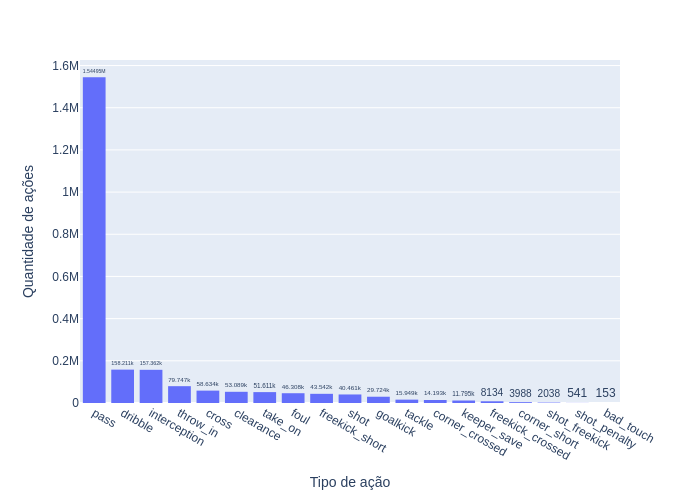
\includegraphics[width=0.5\textwidth]{images/action_distribution.png}
    \caption{Distribuições dos tipos de ação}
    \label{fig:example}
\end{figure}

\subsection{Distribuição da posição de chutes convertidos em gol}



\subsection{Distância média entre passes}

O passe é um dos se não o fundamento mais importante em um esporte coletivo
como o futebol. Uma boa execução desse fundamento por parte dos jogadores
de uma equipe indica um bom controle da posse de bola que está diretamente
conectado com bons resultados \cite{cox2022linhas}. Nesse sentido é
interessante fazer um análise
das distâncias entre os passes
executados por cada equipe.

Em particular, foi coletada a distância entre todos os passes bem sucedidos de
cada equipe e, posteriormente, coletadas estatísticas sobre essas distâncias. A
distância média
entre passes se destacou, uma vez que ela indica como funciona a dinâmica de
troca de passes de uma equipe. Os resultados observados confirmaram suspeitas
prévias acerca do assunto.
Como pode-se notar nas tabelas abaixo, para cada uma das grandes ligas, as
principais equipes, isto é, as equipes com maior grandeza histórica e maior
poderio financeiro figuram como aquelas
que possuem a menor distância média entre passes bem sucedidos. Na Inglaterra,
por exemplo, o Manchester City, equipe comandada pelo espanhol Pep Guardiola,
foi a equipe com a menor média
de distância entre passes. O estilo de jogo de Guardiola é muito focado no
controle da posse de bola e na movimentação dos jogadores para receptar um
passe \cite{terzis2023pep}, então o resultado está dentro do
esperado.

É interessantes notar que os clubes com menor média de distância entre os
passes da temporada 17/18 em cada liga mantiveram posições altas em seus
respectivos campeonatos. O Manchester City e o Paris Saint Germain se sagraram
campeões, enquanto Napoli e Atletico de Madrid ficaram com a segunda colocação.
Na Alemanha, o RB Leipzig ficou com a sexta colocação. Pode-se notar então que
existe uma correlação entre a o desempenho de um time no campeonato com a
distância média entre os passes da equipe.

\begin{table}[H]
    \centering
    \begin{tabular}{|c|c|}
        \hline
        \textbf{Equipe}            & \textbf{Distância média entre passes (m)}
        \\ \hline
        Manchester City FC         & 17.208
        \\ \hline
        Arsenal FC                 & 17.729
        \\ \hline
        Manchester United FC       & 17.823
        \\ \hline
        AFC Bournemouth            & 18.417
        \\ \hline
        Tottenham Hotspur FC       & 18.490
        \\ \hline
        Crystal Palace FC          & 18.555
        \\ \hline
        Chelsea FC                 & 18.682
        \\ \hline
        Southampton FC             & 18.801
        \\ \hline
        Liverpool FC               & 18.808
        \\ \hline
        West Ham United FC         & 18.832
        \\ \hline
        Watford FC                 & 18.967
        \\ \hline
        Newcastle United FC        & 18.972
        \\ \hline
        Swansea City AFC           & 19.077
        \\ \hline
        Leicester City FC          & 19.189
        \\ \hline
        Huddersfield Town FC       & 19.215
        \\ \hline
        Stoke City FC              & 19.690
        \\ \hline
        West Bromwich Albion FC    & 19.712
        \\ \hline
        Everton FC                 & 19.785
        \\ \hline
        Brighton \& Hove Albion FC & 19.838
        \\ \hline
        Burnley FC                 & 20.634
        \\ \hline
    \end{tabular}
    \caption{Premier League}
    \label{tab:average_distance_england}
\end{table}

% Table for the Spanish League
\begin{table}[H]
    \centering
    \begin{tabular}{|c|c|}
        \hline
        \textbf{Equipe}                  & \textbf{Distância média entre passes
            (m)}
        \\ \hline
        Club Atlético de Madrid          & 17.581
        \\ \hline
        FC Barcelona                     & 17.618
        \\ \hline
        UD Las Palmas                    & 17.864
        \\ \hline
        Real Madrid Club de Fútbol       & 17.905
        \\ \hline
        Sevilla FC                       & 18.070
        \\ \hline
        Real Betis Balompié              & 18.659
        \\ \hline
        Villarreal Club de Fútbol        & 18.703
        \\ \hline
        Real Club Deportivo de La Coruña & 18.990
        \\ \hline
        Reial Club Deportiu Espanyol     & 19.018
        \\ \hline
        Real Sociedad de Fútbol          & 19.051
        \\ \hline
        Valencia Club de Fútbol          & 19.090
        \\ \hline
        Deportivo Alavés                 & 19.225
        \\ \hline
        Real Club Celta de Vigo          & 19.324
        \\ \hline
        CD Leganés                       & 19.340
        \\ \hline
        Levante UD                       & 19.353
        \\ \hline
        Málaga Club de Fútbol            & 19.527
        \\ \hline
        Girona FC                        & 20.133
        \\ \hline
        Athletic Club Bilbao             & 20.137
        \\ \hline
        Getafe Club de Fútbol            & 20.608
        \\ \hline
        SD Eibar                         & 20.982
        \\ \hline
    \end{tabular}
    \caption{La Liga}
    \label{tab:average_distance_spain}
\end{table}

% Table for the French League
\begin{table}[H]
    \centering
    \begin{tabular}{|c|c|}
        \hline
        \textbf{Equipe}                          & \textbf{Distância média
        entre passes (m)}                                                  \\
        \hline
        Paris Saint-Germain FC                   & 17.205
        \\ \hline
        O.G.C. Nice Côte d'Azur                  & 17.923
        \\ \hline
        Olympique de Marseille                   & 17.977
        \\ \hline
        Lille OSC Métropole                      & 17.999
        \\ \hline
        En Avant Guingamp                        & 18.008
        \\ \hline
        AS Saint-Étienne                         & 18.320
        \\ \hline
        Olympique Lyonnais                       & 18.377
        \\ \hline
        Angers SCO                               & 18.414
        \\ \hline
        FC Nantes                                & 18.544
        \\ \hline
        Amiens SC                                & 18.570
        \\ \hline
        Espérance Sportive Troyes Aube Champagne & 18.604
        \\ \hline
        FC Girondins de Bordeaux                 & 18.621
        \\ \hline
        AS Monaco FC                             & 19.099
        \\ \hline
        Stade Rennais FC                         & 19.141
        \\ \hline
        FC Metz                                  & 19.266
        \\ \hline
        RC Strasbourg Alsace                     & 19.424
        \\ \hline
        Montpellier HSC                          & 19.592
        \\ \hline
        Toulouse FC                              & 19.677
        \\ \hline
        Stade Malherbe Caen                      & 19.805
        \\ \hline
        Dijon FCO                                & 19.913
        \\ \hline
    \end{tabular}
    \caption{Ligue 1}
    \label{tab:average_distance_france}
\end{table}

% Table for the Italian League
\begin{table}[H]
    \centering
    \begin{tabular}{|c|c|}
        \hline
        \textbf{Equipe}                        & \textbf{Distância média entre
            passes (m)}
        \\ \hline
        SSC Napoli                             & 16.864
        \\ \hline
        FC Internazionale Milano               & 17.370
        \\ \hline
        UC Sampdoria                           & 17.980
        \\ \hline
        AC Milan                               & 18.514
        \\ \hline
        Torino FC                              & 18.564
        \\ \hline
        Benevento Calcio                       & 18.613
        \\ \hline
        ACF Fiorentina                         & 18.654
        \\ \hline
        AC Chievo Verona                       & 18.706
        \\ \hline
        SS Lazio                               & 18.712
        \\ \hline
        Atalanta Bergamasca Calcio             & 18.757
        \\ \hline
        AS Roma                                & 18.759
        \\ \hline
        Società Polisportiva Ars et Labor 2013 & 18.763
        \\ \hline
        Genoa CFC                              & 18.890
        \\ \hline
        Cagliari Calcio                        & 18.897
        \\ \hline
        Juventus FC                            & 18.983
        \\ \hline
        Udinese Calcio                         & 19.043
        \\ \hline
        Bologna FC 1909                        & 19.056
        \\ \hline
        FC Crotone                             & 19.103
        \\ \hline
        Hellas Verona FC                       & 19.202
        \\ \hline
        US Sassuolo Calcio                     & 19.646
        \\ \hline
    \end{tabular}
    \caption{Serie A}
    \label{tab:average_distance_italy}
\end{table}

% Table for the German League

\begin{table}[H]
    \centering
    \begin{tabular}{|c|c|}
        \hline
        \textbf{Equipe}              & \textbf{Distância média entre passes
        (m)}                                                                \\
        \hline
        Rasen Ballsport Leipzig      & 18.123
        \\ \hline
        TSV Bayer 04 Leverkusen      & 18.319
        \\ \hline
        BV Borussia 09 Dortmund      & 18.386
        \\ \hline
        Borussia VfL Mönchengladbach & 18.648
        \\ \hline
        FC Bayern München            & 18.835
        \\ \hline
        TSG 1899 Hoffenheim          & 19.136
        \\ \hline
        FC Schalke 04                & 19.255
        \\ \hline
        Hannover 96                  & 19.269
        \\ \hline
        VfB Stuttgart 1893           & 19.616
        \\ \hline
        1. FC Köln                   & 19.626
        \\ \hline
        Hertha BSC                   & 19.762
        \\ \hline
        Hamburger SV                 & 19.834
        \\ \hline
        VfL Wolfsburg                & 19.836
        \\ \hline
        SV Werder Bremen             & 19.883
        \\ \hline
        1. FSV Mainz 05              & 19.884
        \\ \hline
        SC Freiburg                  & 19.904
        \\ \hline
        FC Augsburg                  & 20.228
        \\ \hline
        Eintracht Frankfurt          & 20.606
        \\ \hline
    \end{tabular}
    \caption{Bundesliga}
    \label{tab:average_distance_germany}
\end{table}

\section{Resultados}

gfdfd

\section{Conclusão}

fefre

\newpage
\bibliographystyle{plain}
\renewcommand{\refname}{Referências Bibliográficas}
\addcontentsline{toc}{section}{Referências Bibliográficas}
\bibliography{sample}
\nocite{*}

\end{document}